\chapter{Распределения, статистики, оценки и введение в гипотезы}
\label{ch:basics}

Курс прикладного статистического анализа данных опирается на три опоры~--- специфические методы для конкретных постановок, границы их применимости и статистическое мышление.
Численные процедуры не превращают таблицу автоматически в научный факт. Если результат противоречит содержательному представлению о данных и не виден на графике, его следует проверить особенно тщательно \citep{marriott1974}.

В настоящей главе закладывается язык всего последующего материала. Речь идёт о случайных величинах и распределениях, выборочных статистиках, точечных и интервальных оценках и проверке гипотез.
С первых страниц полезно возвращаться к трём вопросам из предисловия~--- постановке, применимости и интерпретации~--- и удерживать их в каждой следующей главе.

\section{Случайность, выборка и описательная статистика}
\label{sec:descriptive}

\begin{definition}
Генеральная совокупность~--- множество объектов, свойства которых интересуют в задаче. Выборка $X^n=(X_1,\ldots,X_n)$~--- конечное подмножество, по которому делаются выводы.
\end{definition}

\begin{definition}
Выборка называется простой, если наблюдения независимы и одинаково распределены, i.i.d.
\end{definition}

Основная задача описательной статистики~--- хотя бы приближённо восстановить закон $F_X(x)$ по реализации $x^n$.

\begin{definition}
Статистика $T(X^n)$~--- любая измеримая функция выборки.
\end{definition}

Наиболее часто используются выборочное среднее $\bar X=\frac1n\sum X_i$, несмещённая выборочная дисперсия $S^2=\frac1{n-1}\sum(X_i-\bar X)^2$, вариационный ряд $X_{(1)}\le\cdots\le X_{(n)}$ и производные от него квантили и медиана.

Одной средней или дисперсии недостаточно для описания распределения.
Среднее, медиана и мода в общем случае не совпадают. Для мультимодальных или асимметричных данных одно число $\bar x$ может вводить в заблуждение.
Перед выбором метода всегда строят гистограммы, ящики с усами и эмпирическую функцию распределения.
Полезно мысленно пройти маршрут от сырых чисел к выводу на одном наборе данных. Сначала оценить симметрию, выбросы и моды, затем выбрать центральную меру и меру разброса и только после этого решать, уместен ли параметрический критерий из следующих глав.
Такая последовательность не требует новых формул~--- она дисциплинирует интерпретацию. Если график противоречит среднему, доверять среднему нельзя, даже при малом p-value.
Статистика в прикладном смысле~--- это сжатое описание выборки, а не самодостаточный вывод из одной ячейки таблицы. Она должна отражать тот аспект распределения, который важен для вопроса исследования — центра, разброса и формы хвостов.
Если вопрос касается типичного значения при симметричных данных~--- достаточно $\bar x$. Если данные асимметричны или с выбросами~--- медиана и квантили информативнее, а среднее может вводить в заблуждение. Непараметрические критерии главы~\ref{ch:hypothesis} дают ту же картину для асимметричных распределений.

Квартет Энскомба \citep{anscombe1973}~--- четыре пары выборок $(x_i,y_i)$, у которых совпадают выборочные средние, дисперсии и корреляция с точностью до округления.

\begin{center}
\footnotesize
\begin{tabular}{|>{$}l<{$}|>{$}c<{$}|>{$}c<{$}|>{$}c<{$}|>{$}c<{$}|}
\hline
\text{№} & 1 & 2 & 3 & 4 \\ \hline
\bar{x} & 9 & 9 & 9 & 9 \\ \hline
S_x & 11 & 11 & 11 & 11 \\ \hline
\bar{y} & 7{,}5 & 7{,}5 & 7{,}5 & 7{,}5 \\ \hline
S_y & 4{,}127 & 4{,}127 & 4{,}128 & 4{,}128 \\ \hline
r_{xy} & 0{,}816 & 0{,}816 & 0{,}816 & 0{,}816 \\ \hline
\end{tabular}
\end{center}

Таблица создаёт впечатление одинаковых данных, тогда как на графиках на рис.~\ref{fig:anscombe} видны линейная зависимость, нелинейность, выброс и вертикальная полоса точек. Отсюда следует, что на сводные числа без визуализации полагаться нельзя.
Типичная ошибка~--- сравнить сводные статистики по нескольким проектам, заключить об их идентичности и объединить отчёт.
Квартет Энскомба показывает, что такое решение может быть содержательно неверным. В одном случае нужна линейная регрессия, в другом~--- полиномиальная, в третьем~--- робастная процедура из-за выброса. Совпадение $\bar x$, $S_x$ и $r_{xy}$ не означает, что выборки описывают одну и ту же предметную ситуацию или порождены одной моделью.

\begin{figure}[htbp]
    \centering
    
\includegraphics[width=\FigWidth]{{figures/chapter-1/Anscombe's_quartet}}
    \caption{Квартет Энскомба. Одинаковые $\bar x$, $S_x$, $\bar y$, $S_y$, $r_{xy}$ при разной геометрии.}
    \label{fig:anscombe}
\end{figure}

Набор ирисов Фишера содержит четыре морфологических признака трёх видов ирисов. На рис.~\ref{fig:iris-box} показано, что среднее, медиана и мода в общем случае не совпадают, а разные виды дают разные центры распределений.

\begin{figure}[htbp]
    \centering
    
\includegraphics[width=\FigWidth]{\FigDir/chapter-1/mmm.png}
    \caption{Среднее, медиана и мода. Различие центральных характеристик.}
    \label{fig:iris-box}
\end{figure}

\section{Эмпирическая функция распределения и оценка плотности}

\begin{definition}
Эмпирическая функция распределения, ЭФР, для выборки $X^n$ задаётся как
\[ F_n(x)=\frac1n\sum_{i=1}^n [X_i\le x].
\]
Это статистика, оценивающая $F(x)$. По закону больших чисел $F_n(x)\to F(x)$ при $n\to\infty$.
\end{definition}

\begin{definition}
Оценка плотности строится по выборке ядерным сглаживанием или гистограммой и приближает истинную плотность $f(x)$.
\end{definition}

Для синтетической нормальной выборки ЭФР приведена на рис.~\ref{fig:ecdf}, оценка плотности~--- на рис.~\ref{fig:iris-hist}. Сглаженная плотность может выявлять мультимодальность, скрытую за $\bar x$.

\begin{figure}[htbp]
    \centering
    
\includegraphics[width=\FigWidth]{\FigDir/chapter-1/epdf.png}
    \caption{Оценка плотности распределения по выборке.}
    \label{fig:iris-hist}
\end{figure}

\begin{figure}[htbp]
    \centering
    
\includegraphics[width=\FigWidth]{\FigDir/chapter-1/ecdf.png}
    \caption{Эмпирическая функция распределения.}
    \label{fig:ecdf}
\end{figure}

ЭФР и оценка плотности не заменяют параметрическую модель, но задают эмпирическую картину данных без предположений о семействе $F$.
На одном рисунке удобно совместить гистограмму, ядерную оценку плотности и ЭФР в отдельных панелях~--- так видно, совпадает ли форма с предполагаемой моделью. Ступень ЭФР в точке $x_0$ равна доле наблюдений $\le x_0$, резкий скачок указывает на кластер значений, который гистограмма с грубым числом корзин может размазать.
ЭФР и оценку плотности используют при первичном анализе, при построении критериев согласия в гл.~\ref{ch:hypothesis} и как основу бутстрепа. Псевдовыборки с возвращением эквивалентны сэмплированию из $F_n$. Ступенчатая ЭФР показывает накопленные вероятности, сглаженная плотность~--- локальные особенности вроде мод и асимметрии.
Для одной числовой переменной типична такая последовательность. Строят гистограмму и ЭФР. Если форма близка к колоколу и выбросов нет, приводят $\bar x$ и $S$ и планируют $t$-интервал. Если хвост тяжёлый, добавляют медиану, квантили и готовят ранговый критерий в гл.~\ref{ch:hypothesis}. На одном графике сразу видно, уместна ли нормальная модель или нужна робастная альтернатива.

\section{Распределения случайных величин}

\begin{definition}
Дискретная с.\,в.\ задаётся функцией вероятности $f_X(a_i)=\prob(X=a_i)$. Непрерывная~--- функцией распределения $F_X(x)=\prob(X\le x)$ или плотностью $f_X$, для которой $\prob(a\le X\le b)=\int_a^b f_X(x)\,dx$.
\end{definition}

В прикладной статистике снова и снова встречаются несколько параметрических семейств. Нормальное распределение и законы, производные от него ($\chi^2$, Стьюдента, Фишера), получают точный вывод при проверке средних и дисперсий. Биномиальное и распределение Пуассона естественны для бинарных и редких счётных наблюдений. Связи между этими семействами, в частности $Z/\sqrt{V/\nu}\sim St(\nu)$, объясняют появление именно этих законов в формулах критериев.

Среди непрерывных семейств центральное место занимает нормальное $N(\mu,\sigma^2)$, $\sigma^2>0$. \[ f(x)=\frac1\sigma\phi\!\left(\frac{x-\mu}{\sigma}\right),\quad F(x)=\Phi\!\left(\frac{x-\mu}{\sigma}\right), \] где $\phi$, $\Phi$~--- плотность и функция распределения $N(0,1)$.
Для него $\mathbb EX=\med X=\mu$, $\mathbb DX=\sigma^2$, линейная комбинация нормальных снова нормальна. ЦПТ утверждает, что при i.i.d.\ с конечной дисперсией $\bar X_n \approx N\!\bigl(\mathbb EX,\mathbb DX/n\bigr)$ при большом $n$.

$\chi^2_k$. Если $Z_1,\ldots,Z_k$ i.i.d.\ $N(0,1)$, то $\sum_{i=1}^k Z_i^2\sim\chi^2_k$. \[ f(x)=\frac{1}{2^{k/2}\Gamma(k/2)}\,x^{k/2-1}e^{-x/2},\quad x>0.
\] При $X_i\sim N(\mu,\sigma^2)$ величина $(n-1)S^2/\sigma^2$ имеет распределение $\chi^2_{n-1}$.

Стьюдента $St(\nu)$. $T=Z/\sqrt{V/\nu}$, $Z\sim N(0,1)$, $V\sim\chi^2_\nu$ независимы. \[ f(t)=\frac{\Gamma\bigl(\frac{\nu+1}{2}\bigr)}{\sqrt{\nu\pi}\,\Gamma\bigl(\frac{\nu}{2}\bigr)} \left(1+\frac{t^2}{\nu}\right)^{-(\nu+1)/2}.
\] При $\nu\to\infty$ распределение сходится к $N(0,1)$.

Фишера $F(d_1,d_2)$. $F=\dfrac{X_1/d_1}{X_2/d_2}$, $X_i\sim\chi^2_{d_i}$ независимы. Возникает в ANOVA и сравнении дисперсий.
\begin{figure}[htbp]
    \centering
    \begin{subfigure}[b]{\FigWidth}
        \centering
        
\includegraphics[width=\linewidth]{\FigDir/chapter-1/norm.png}
        \caption{Нормальное $N(0,1)$}
    \end{subfigure}\\[0.6em]
    \begin{subfigure}[b]{\FigWidth}
        \centering
        
\includegraphics[width=\linewidth]{\FigDir/chapter-1/chi2.png}
        \caption{$\chi^2_k$ при разных $k$}
    \end{subfigure}\\[0.6em]
    \begin{subfigure}[b]{\FigWidth}
        \centering
        
\includegraphics[width=\linewidth]{\FigDir/chapter-1/stud.png}
        \caption{Стьюдента $St(\nu)$}
    \end{subfigure}
    \caption{Плотности нормального, $\chi^2$ и Стьюдента~--- распределения, из которых
 складываются $t$-, $F$- и $\chi^2$-критерии.}
    \label{fig:cont-dists}
\end{figure}

\begin{figure}[htbp]
    \centering
    
\includegraphics[width=\FigWidth]{\FigDir/chapter-1/fish.png}
    \caption{Распределение Фишера при разных числах степеней свободы.}
    \label{fig:fish}
\end{figure}

Для дискретных наблюдений естественны Бернулли $Ber(p)$, $p\in(0,1)$. Случайная величина $X\in\{0,1\}$, \[ \prob(X=1)=p,\quad \prob(X=0)=1-p.
\]

Биномиальное $Bin(N,p)$ описывает число успехов в $N$ независимых испытаниях. \[ \prob(X=k)=C_N^k p^k(1-p)^{N-k},\quad k=0,\ldots,N.
\] Если $X_i\sim Ber(p)$ i.i.d., то $\sum X_i\sim Bin(n,p)$.
При $N>20$ и $p$, отличном от нуля и единицы, возможна нормальная аппроксимация.

Пуассона $Pois(\lambda)$, $\lambda>0$. \[ \prob(X=k)=e^{-\lambda}\frac{\lambda^k}{k!},\quad k=0,1,2,\ldots, \quad \mathbb EX=\mathbb DX=\lambda.
\] Моделирует число редких независимых событий в интервале. При $n\to\infty$, $np\to\lambda$ выполняется $Bin(n,p)\to Pois(\lambda)$.
Связь биномиального и Пуассона часто используют на практике как эвристику выбора модели. Если $n$ велико, а $p$ мало, биномиальное распределение близко к Пуассоновскому с тем же $\lambda=np$, и формулы упрощаются. Обратная ситуация~--- малые $n$ и $p$ у края $(0,1)$~--- требует точного биномиального критерия из гл.~\ref{ch:hypothesis}, а не нормальной аппроксимации по привычке.
\begin{figure}[htbp]
    \centering
    \begin{subfigure}[b]{\FigWidth}
        \centering
        
\includegraphics[width=\linewidth]{\FigDir/chapter-1/ber.png}
        \caption{Бернулли}
    \end{subfigure}\\[0.6em]
    \begin{subfigure}[b]{\FigWidth}
        \centering
        
\includegraphics[width=\linewidth]{\FigDir/chapter-1/bin.png}
        \caption{Биномиальное}
    \end{subfigure}\\[0.6em]
    \begin{subfigure}[b]{\FigWidth}
        \centering
        
\includegraphics[width=\linewidth]{\FigDir/chapter-1/poiss.png}
        \caption{Пуассона}
    \end{subfigure}
    \caption{Дискретные распределения для счётных и бинарных данных.}
    \label{fig:disc-dists}
\end{figure}

Нормальность~--- рабочая модель, а не свойство реальных данных.
Тяжёлые хвосты и асимметрия нарушают выводы t-критерия и доверительных интервалов, построенных только на ЦПТ.
Для счётных данных сначала проверяют применимость Пуассона или биномиальной модели, а не нормальную аппроксимацию по умолчанию.
При переходе от описательной статистики к параметрическим распределениям полезно выстраивать последовательность шагов. Гистограмма $\to$ гипотеза о семействе $F$ $\to$ оценка параметров $\to$ проверка согласия.
Если на первом шаге видны две моды или тяжёлый хвост, нормальное распределение может служить лишь грубым приближением для $\bar X$ при большом $n$, но не оправдывает $t$-критерий на малых выборках без диагностики.

\section{Описательные статистики и робастность}

Среднее и дисперсия, введённые в разд.~\ref{sec:descriptive}, описывают центр и разброс, но не фиксируют форму распределения. Здесь количественно вводятся асимметрия, эксцесс и робастные меры центра, которые определяют выбор между $\bar x$ и медианой при построении интервалов и критериев.

Медиана и квантили устойчивее среднего к выбросам. Мода полезна при мультимодальных данных. Коэффициент асимметрии \[ \gamma_1 = \mathbb{E}\left(\frac{X-\mathbb{E}X}{\sqrt{\mathbb{D}X}}\right)^3 \] и коэффициент эксцесса \[ \gamma_2 = \frac{\mathbb{E}(X-\mathbb{E}X)^4}{(\mathbb{D}X)^2}-3 \] описывают скошенность и тяжесть хвостов. Условие $\gamma_1=0$ необходимо, но не достаточно для симметрии, см.~рис.~\ref{fig:skew-kurt}.
Коэффициенты $\gamma_1$ и $\gamma_2$ удобны для количественного сравнения с нормалью, но не заменяют визуальный осмотр. Распределение может быть симметричным по $\gamma_1$ и при этом иметь мультимодальность или локальные аномалии, невидимые в двух числах.
На практике робастность~--- это не замена среднего медианой во всех случаях, а осознанный выбор. Если выбросы содержательны как реальный экстремальный случай, их нельзя исключить из анализа только статистикой. Если это ошибки измерения, медиана и квантили дают устойчивую картину центра и разброса.
Сравнение $\bar x$ и медианы на одном графике часто быстрее любого формального теста на асимметрию. Расхождение на 10--20\% при умеренном $n$ уже сигнал, что $t$-интервал для среднего может вводить в заблуждение.

\begin{figure}[htbp]
    \centering
    \begin{subfigure}[b]{\FigWidth}
        \centering
        
\includegraphics[width=\linewidth]{\FigDir/chapter-1/skewness.png}
        \caption{Асимметрия по $\gamma_1$}
    \end{subfigure}\\[0.6em]
    \begin{subfigure}[b]{\FigWidth}
        \centering
        
\includegraphics[width=\linewidth]{\FigDir/chapter-1/kurtosis.png}
        \caption{Эксцесс по $\gamma_2$}
    \end{subfigure}
    \caption{Форма распределения относительно нормального. Скошенность и тяжесть хвостов.}
    \label{fig:skew-kurt}
\end{figure}

\section{Точечное и интервальное оценивание}

\begin{definition}
Пусть $F(x)=F(x,\theta)$. Статистика $\hat\theta_n=\hat\theta(X^n)$ называется точечной оценкой неизвестного параметра $\theta$.
\end{definition}

\begin{definition}
Оценка $\hat\theta_n$ называется состоятельной, если $\plim\hat\theta_n=\theta$. Она несмещённа, если $\mathbb{E}\hat\theta_n=\theta$. Среди несмещённых оценок эффективной называют оценку с минимальной дисперсией.
\end{definition}

Ни одно свойство не выполняется изолированно от постановки. Несмещённая оценка может иметь большую дисперсию, состоятельная на малых $n$ может быть смещённой, как $\hat\sigma^2_{MLE}$ с делителем $n$ вместо $n-1$. Выбор оценки зависит от постановки и формы данных, а не от абстрактной таблицы достоинств.

\begin{definition}
Пусть $X_i\sim f(x,\theta)$ i.i.d. Функция правдоподобия $L(\theta)=\prod_i f(X_i,\theta)$, логарифм правдоподобия $\ell(\theta)=\sum_i \log f(X_i,\theta)$. Оценка максимального правдоподобия, ОМП, $\hat\theta_{MLE}=\argmax_\theta \ell(\theta)$ удовлетворяет уравнению правдоподобия $S(\theta)=\partial\ell/\partial\theta=0$.
\end{definition}

Для $X_i\sim N(\mu,\sigma^2)$ при известной $\sigma^2$ из $S(\mu)=0$ получают $\hat\mu_{MLE}=\bar X$. При неизвестной $\sigma^2$ величина $\hat\sigma^2_{MLE}=\frac1n\sum(X_i-\bar X)^2$ смещена, несмещённой служит $S^2$ с делителем $n-1$. Для $X_i\sim Ber(p)$ аналогично $\hat p_{MLE}=\bar X$. При стандартных регулярных условиях ОМП состоятельна, асимптотически нормальна и эффективна, а $g(\hat\theta_{MLE})$ является ОМП для $g(\theta)$.

ОМП выбирает параметры, при которых наблюдённые данные наиболее правдоподобны, но не освобождает от проверки модели. При неверном семействе $f(\cdot,\theta)$ она остаётся лучшей оценкой внутри неправильного класса распределений, поэтому оценивание всегда сопровождают графиками и критериями согласия в гл.~\ref{ch:hypothesis}. Для нормальной выборки $\hat\mu_{MLE}=\bar x$, 95\%-й $t$-интервал для $\mu$ и одновыборочный $t$-критерий $H_0\colon\mu=\mu_0$ используют одну и ту же стандартизацию. Если Q--Q график противоречит $N(\mu,\sigma^2)$, пересматривают все три вывода, а не только p-value.

\begin{definition}
Интервал $[C_L,C_U]$ называется доверительным уровня $1-\alpha$, если $\prob(\theta\in[C_L,C_U])\ge 1-\alpha$ как свойство процедуры построения, а не отдельного числового отрезка для данной выборки.
\end{definition}

Корректная частотная интерпретация такова. При многократном повторении эксперимента с тем же $n$ и той же процедурой примерно $(1-\alpha)\cdot 100\%$ построенных интервалов накроют $\theta$. Это не утверждение о том, что «параметр с вероятностью $1-\alpha$ лежит в уже построенном интервале». Та же логика отличает доверительный интервал от байесовского достоверного интервала в гл.~\ref{ch:bayes}.

Для $N(\mu,\sigma^2)$ при известной $\sigma$ \[ \bar X \pm z_{1-\alpha/2}\,\frac{\sigma}{\sqrt n}.
\] При неизвестной $\sigma$ и нормальных данных берут $t_{n-1}$, для больших $n$ и произвольных $F$~--- приближение по ЦПТ с заменой $\mathbb DX$ на $S^2$. При малых $n$ замена $t$ на $z$ при неизвестной дисперсии может завышать уверенность.

\begin{definition}
Бутстреп \citep{efron1979,efron1993} строит эмпирическое распределение статистики $\hat\theta^{*}$ по $N$ псевдовыборкам объёма $n$, взятых из исходных данных с возвращением. Доверительный интервал получают по квантилям этого распределения, по студентизированной формуле или по поправке BCa.
\end{definition}

Схема бутстрепа на рис.~\ref{fig:boot} напрямую связана с ЭФР. Псевдовыборка с возвращением~--- новая реализация из $F_n$. Наивный перцентильный интервал берёт квантили порядка $\alpha/2$ и $1-\alpha/2$ бутстреп-распределения $\hat\theta^{*}$. Бутстреп полезен, когда аналитический закон $T(X^n)$ неизвестен, но не исправляет неверную модель и плохо работает для статистик, определяемых малым числом наблюдений, например для медианы при $n=15$. Число псевдовыборок $N$ задаёт точность оценки квантилей, а не заменяет рост $n$. Схему на данных семинара см. в разд.~\ref{sec:practice-ch1}.

\begin{figure}[htbp]
    \centering
    
\includegraphics[width=\FigWidth]{\FigDir/chapter-1/boot3.png}
    \caption{Схема бутстрепа. Псевдовыборки и бутстреп-распределение статистики.}
    \label{fig:boot}
\end{figure}

Полный каталог параметрических и непараметрических критериев, критериев согласия и асимптотических процедур развивается в главе~\ref{ch:hypothesis}.
В настоящей главе закрепляются язык проверки гипотез (p-value, ошибки I и II рода, мощность, размер эффекта) и типичные ошибки интерпретации.
При чтении курса подряд сначала освойте этот блок, затем перейдите к выбору конкретной статистики $T$ и её нулевому распределению.

\section{Введение в проверку гипотез}

\begin{definition}
Статистическая гипотеза~--- утверждение о распределении или его параметрах. $H_0$~--- нулевая гипотеза, $H_1$~--- альтернатива. p-value~--- вероятность при $H_0$ получить значение статистики $T$ не менее экстремальное, чем наблюдаемое $T_{\text{obs}}$. Что считать экстремальным, задаёт $H_1$.
\end{definition}

$H_0$ нельзя отвергать механически по одному только сравнению с порогом $\alpha$. Если p-value $<\alpha$, гипотезу отвергают на уровне $\alpha$, но p-value $\neq\prob(H_0)$. Пример осьминога, угадавшего 11 из 13 исходов, даёт p-value $\approx 0{,}011$, хотя при верной $H_0$ говорить об угадывании наугад некорректно.

\begin{definition}
Ошибка I рода~--- ложное отвержение $H_0$, её вероятность равна уровню значимости $\alpha$. Ошибка II рода~--- неотвержение $H_0$ при истинной $H_1$, $\beta=\prob(\text{не отвергнуть}\mid H_1)$. Мощность критерия $1-\beta$~--- вероятность отвергнуть $H_0$, когда верна $H_1$.
\end{definition}

Мощность растёт с $n$, с величиной отклонения от $H_0$ и с чувствительностью статистики. При планировании эксперимента задают минимальный размер эффекта $\delta$ и требуемую мощность, часто $1-\beta=0{,}8$, по кривым мощности подбирают $n$ до сбора данных. Слишком маленькая выборка ведёт к частым ошибкам II рода, слишком большая~--- к отвержению $H_0$ при несущественных отличиях.

p-value отражает совместимость наблюдения с $H_0$, но не измеряет величину эффекта. С ростом $n$ даже микроскопические отклонения становятся статистически значимыми, поэтому всегда оценивают размер эффекта в единицах предметной области. Три характерных ситуации иллюстрируют различие статистической и содержательной значимости.

\begin{itemize}
 \item Исследование физической активности Lee et al., 2010. При p-value $<0{,}001$
 разница в наборе веса за три года составила 150~г~--- статистически значимо, практическая польза сомнительна.
 \item Клинические испытания. Рост риска инфаркта на 0{,}07\% может быть
 малым для одного человека, но при массовом применении препарата~--- тысячи дополнительных случаев.
 \item Исследование при болезни Альцгеймера. Разница в IQ на 13 пунктов
 может быть клинически важной даже при p-value $>\alpha$ на малой выборке~--- имеет смысл увеличить $n$, а не только смотреть на p-value.
\end{itemize}

При интерпретации тестов повторяются типичные ошибки.

\begin{itemize}
 \item Путать p-value с вероятностью истинности $H_0$.
 \item Считать p-value, близкий к порогу $\alpha$, доказательством отсутствия эффекта.
 Отсутствие доказательств не равно доказательству отсутствия.
 \item Проводить множество тестов без поправки, см.~гл.~\ref{ch:multiple}.
 \item Выбирать одностороннюю альтернативу после просмотра данных.
\end{itemize}

Завершающий пример главы связывает введённые блоки. Для времени отклика службы поддержки при $n=120$ гистограмма и ЭФР показывают правоскошение и пик у нуля. Среднее $\bar x=42{,}3$~с и медиана $18$~с дают разную типичную картину. Q--Q график отклоняется на хвостах, при нормальной модели 95\%-й $t$-интервал для $\mu$ равен $[35{,}1,\,49{,}5]$, проверка $H_0\colon\mu=30$~с даёт p-value $\approx 0{,}002$. Интерпретация требует и p-value, и медианы, и, при необходимости, бутстреп-интервала для робастного центра. SLA по среднему и по медиане~--- разные KPI, статистика обязана показать обе картины.

К любой сводной статистике полезно вернуться к трём вопросам из предисловия. Репрезентативна ли выборка? Не вводит ли одно число в заблуждение из-за формы распределения? Подходит ли выбранная мера для описания, интервала или теста? Если форма сомнительна, переходят к робастным и непараметрическим методам гл.~\ref{ch:hypothesis}, не меняя $\alpha$ постфактум.

\section{Непараметрические интервалы, BCa-бутстреп и мощность критерия}

Для медианы и произвольного квантиля непрерывного распределения существуют точные непараметрические интервалы по порядковым статистикам. Они дополняют параметрические интервалы для $\mu$ при нормальности и перцентильный бутстреп, введённый ранее в этой главе.

Пусть $X^n=(X_1,\ldots,X_n)$, $X_{(1)}\le\cdots\le X_{(n)}$~--- вариационный ряд.
Для медианы $\med X$ при непрерывном $F$ \[ \prob\bigl(\med X \in [X_{(r)},\, X_{(n-r+1)}]\bigr) =\frac1{2^n}\sum_{i=r}^{n-r+1} C_n^i.
\] Индексы $r$ и $n-r+1$ подбирают так, чтобы эта вероятность была $\ge 1-\alpha$. При дискретности распределения порядковых статистик интервал может быть чуть консервативнее.

При $n>10$ удобна нормальная аппроксимация \[ \prob\Bigl(\med X \in \Bigl[ X_{\bigl(\lfloor (n-\sqrt{n}\,z_{1-\alpha/2})/2\rfloor\bigr)},\, X_{\bigl(\lceil (n+\sqrt{n}\,z_{1-\alpha/2})/2\rceil\bigr)} \Bigr]\Bigr) \approx 1-\alpha.
\]

Аналогично для $\alpha$-квантиля $X_\alpha$, $\alpha\in(0,1)$, \[ \prob\bigl(X_\alpha \in [X_{(l)},\, X_{(u)}]\bigr) =\sum_{i=l}^{u} C_n^i\,\alpha^i(1-\alpha)^{n-i}.
\] Границы $l$ и $u$ выбирают по той же логике покрытия $1-\alpha$.
На практике такие интервалы особенно полезны при асимметрии и выбросах, когда $t$-интервал для $\bar X$ вводит в заблуждение.

Для BCa-бутстрепа \citep{efron1993} пусть $\hat\theta_n=\hat\theta(X^n)$~--- оценка параметра, $X^{1*},\ldots,X^{N*}$~--- $N$ псевдовыборок с возвращением объёма $n$, $\hat\theta_n^{i*}$~--- значения статистики на них, $F_{\hat\theta_n}^{\mathrm{boot}}$~--- их эмпирическая функция распределения.
 Несмещённый ускоренный BCa доверительный интервал уровня $1-\alpha$ задаётся как \[ \prob\Bigl( \bigl(F_{\hat\theta_n}^{\mathrm{boot}}\bigr)^{-1}(\alpha_1) \le \theta \le \bigl(F_{\hat\theta_n}^{\mathrm{boot}}\bigr)^{-1}(\alpha_2) \Bigr)\approx 1-\alpha, \] где
\begin{align*}
\alpha_1 &= \Phi\!\left(
\hat{z}_0 + \frac{\hat{z}_0 + z_{\alpha/2}}{1 - \hat{a}\,(\hat{z}_0 + z_{\alpha/2})}
\right), \\
\alpha_2 &= \Phi\!\left(
\hat{z}_0 + \frac{\hat{z}_0 + z_{1-\alpha/2}}{1 - \hat{a}\,(\hat{z}_0 + z_{1-\alpha/2})}
\right), \\
\hat{z}_0 &= \Phi^{-1}\!\left(
\frac1N\sum_{i=1}^N \mathbf{1}\bigl[\hat\theta_n^{i*} < \hat\theta_n\bigr]
\right).
\end{align*}
Поправка смещения $\hat{z}_0$ сдвигает квантили бутстреп-распределения с учётом асимметрии. Параметр ускорения $\hat{a}$ оценивают по джекнайфу при последовательном исключении одного наблюдения, \[ \hat{a} =\frac{\sum_{i=1}^n (\bar{\theta}_{(\cdot)}-\theta_{(i)})^3} {6\left[\sum_{i=1}^n (\bar{\theta}_{(\cdot)}-\theta_{(i)})^2\right]^{3/2}}, \quad \bar{\theta}_{(\cdot)}=\frac1n\sum_{i=1}^n\theta_{(i)}, \] где $\theta_{(i)}$~--- значение $\hat\theta$ на выборке без $i$-го элемента.
BCa часто точнее наивного перцентильного интервала при смещённых и асимметричных бутстреп-распределениях.

Количественную иллюстрацию мощности и ошибок II рода даёт классический пример теста Джеймса Бонда на предпочтение взболтанного мартини.
Пусть ненаблюдаемая вероятность выбора взболтанного мартини равна $51\%$. После $100$ испытаний взболтанный выбран $49$ раз. Для односторонней альтернативы о предпочтении взболтанного мартини p-value $\approx 0{,}62$~--- $H_0$ не отвергается, хотя мартини выбирают несимметрично.

При истинной вероятности $75\%$ и критерии на долю успехов с двусторонней альтернативой и отвержением при экстремальных $t$ мощность при $n=100$ составляет лишь $(1-\beta)\approx 0{,}62$. Даже при заметном отклонении от $H_0$ критерий пропустит эффект в $\approx 38\%$ повторений эксперимента. Отсюда следует необходимость планирования выборки до сбора данных. Фиксируют минимальный детектируемый эффект, например $p\ge 0{,}75$, и требуемую мощность $1-\beta$, часто $0{,}8$, по кривым мощности подбирают $n$. Статистическая мощность и содержательная постановка риска здесь неразделимы.

\section{Практика и семинар}
\label{sec:practice-ch1}


\PracticeIntro{1}
Данные Boston Housing: медианная стоимость жилья и признаки районов (набор семинара~1).

\paragraph{Boston: распределение \texttt{medv}.}
\textbf{Данные и вопрос.} $n=506$ наблюдений, отклик \texttt{medv} --- медианная стоимость жилья (тыс.\ долл.).
Вопрос семинара: каков типичный уровень цен и насколько разброс велик; уместен ли $t$-интервал для среднего?

\textbf{График.} Гистограмма и boxplot (рис.~\ref{fig:p1-shape}) показывают правоскошение и плотный хвост дорогих районов.
На графике видно: медиана ниже среднего, выбросы справа --- среднее чувствительно к элитным районам.

\begin{figure}[htbp]
\centering
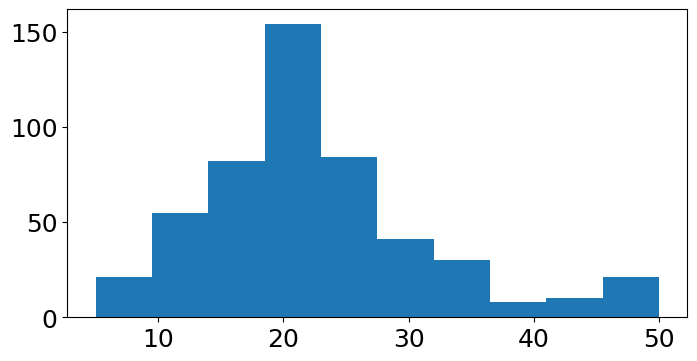
\includegraphics[width=\FigWidth]{figures/practice/chapter-1/sem1-cell36-out0.png}
\caption{Семинар~1: \texttt{medv}. Обратите внимание на правоскошение и отдельные дорогие наблюдения в хвосте.}
\label{fig:p1-shape}
\end{figure}

\begin{figure}[htbp]
\centering
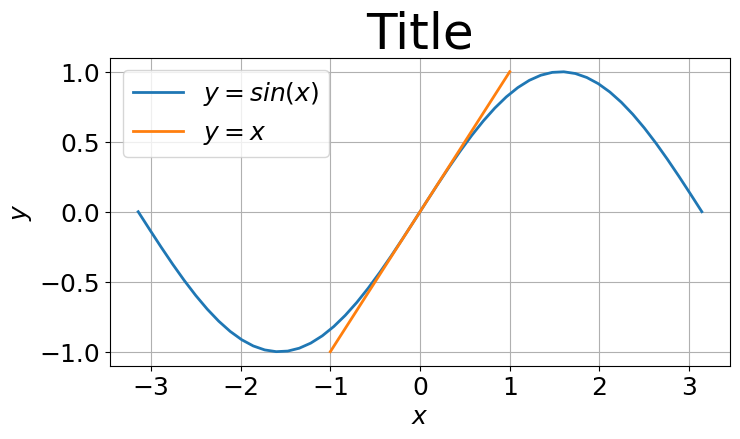
\includegraphics[width=\FigWidth]{figures/practice/chapter-1/sem1-cell09-out0.png}
\caption{Семинар~1: эмпирическая функция распределения \texttt{medv}. На графике видно пологий подъём в левой части и длинный хвост справа.}
\label{fig:p1-ecdf}
\end{figure}

\textbf{Метод и числа.} $\bar x\approx 22{,}5$, медиана $\approx 21{,}2$, $s\approx 9{,}2$.
95\%-й $t$-интервал для $\mathbb E X$: примерно $[20{,}2,\,24{,}8]$; перцентильный бутстреп для $\bar x$ даёт близкий интервал (схема --- рис.~\ref{fig:boot} выше).

\medskip\noindent\textbf{Три вопроса.} \textit{Постановка:} цена жилья в выборке Boston, одна непрерывная переменная.
\textit{Применимость:} сначала форма распределения (гистограмма, ECDF); $t$-ДИ --- при умеренной асимметрии как приближение, медиана и бутстреп --- при сомнении.
\textit{Вывод:} типичная цена около 21--22 тыс.; разброс большой; в отчёте указать асимметрию и не трактовать $t$-ДИ как точный для сильно скошенных данных.\medskip
\paragraph{Связь \texttt{medv} с \texttt{lstat}.}
\textbf{Данные и вопрос.} Предиктор \texttt{lstat} --- доля населения низкого соц.\ статуса; ожидаем отрицательную связь с ценой.

\textbf{График.} Диаграмма рассеяния (рис.~\ref{fig:p1-scatter}) --- почти линейное падение; на pairplot по числовым признакам (рис.~\ref{fig:p1-pair}) видно, что \texttt{lstat} сильнее прочих коррелирует с \texttt{medv}.

\begin{figure}[htbp]
\centering
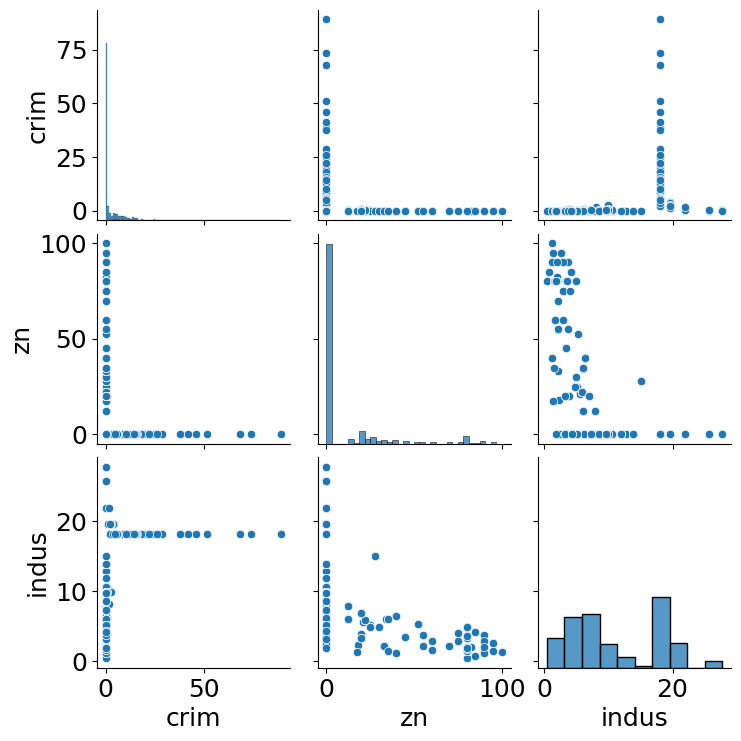
\includegraphics[width=\FigWidth]{figures/practice/chapter-1/sem1-cell45-out0.png}
\caption{Семинар~1: \texttt{medv} и \texttt{lstat}. На графике видно монотонное снижение цены при росте \texttt{lstat}.}
\label{fig:p1-scatter}
\end{figure}
\begin{figure}[htbp]
\centering
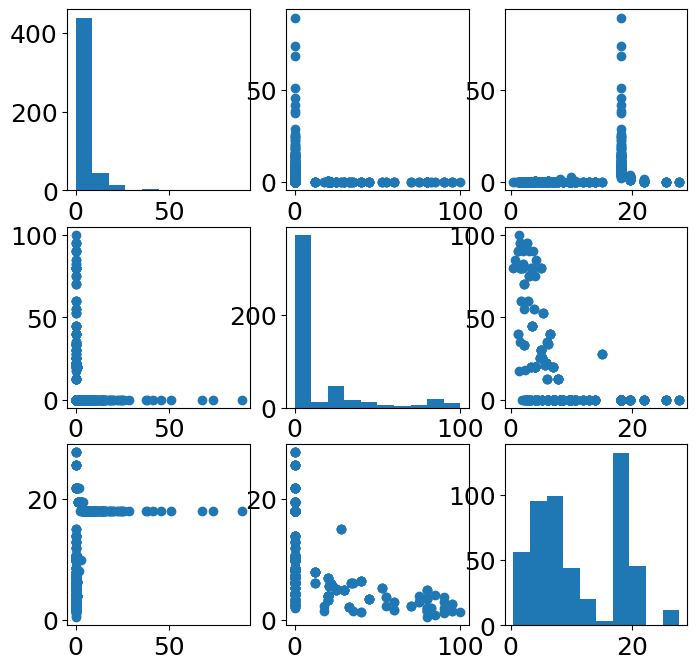
\includegraphics[width=\FigWidth]{figures/practice/chapter-1/sem1-cell47-out0.png}
\caption{Семинар~1: pairplot числовых признаков. Обратите внимание на насыщенный столбец/строку для \texttt{medv}--\texttt{lstat}.}
\label{fig:p1-pair}
\end{figure}

\medskip\noindent\textbf{Три вопроса.} \textit{Постановка:} две непрерывные переменные, исследуем ассоциацию, не причинность.
\textit{Применимость:} scatter и корреляция Пирсона после визуального осмотра; при выбросах --- Спирмен (гл.~\ref{ch:anova}).
\textit{Вывод:} чем выше \texttt{lstat}, тем ниже \texttt{medv}; для отчёта нужна регрессия (гл.~\ref{ch:regression}), здесь --- разведка.\medskip
\paragraph{Домашнее задание sem1.}
Персональная выборка по почте: шаги те же (график $\to$ центр/разброс $\to$ интервал), числа свои; сверяйте форму распределения с рис.~\ref{fig:p1-shape}, а не только с $\bar x$.
\medskip\noindent\textbf{Три вопроса.} \textit{Постановка:} своя непрерывная переменная из задания.
\textit{Применимость:} гистограмма или ECDF, затем центр и ДИ; при асимметрии --- медиана и бутстреп (гл.~\ref{ch:basics}).
\textit{Вывод:} типичный уровень, разброс и оговорка о форме; не цитировать только $\bar x$ без графика.\medskip

По итогам раздела: для каждой задачи --- объекты измерения, график, процедура, 1--3 числа, вывод словами; типичная ошибка --- $t$-интервал при сильной асимметрии без проверки формы.

\section{Контрольные вопросы по теме}

\begin{enumerate}
 \item Чем отличается доверительный интервал от байесовского достоверного интервала, см.~гл.~\ref{ch:bayes}?
 \item Почему выборочная медиана робастнее среднего?
 \item Запишите функцию правдоподобия для $Bin(n,p)$ и ОМП $\hat p$.
 \item Выведите $\hat\mu_{MLE}$ для нормальной выборки через $S(\mu)=0$.
 \item Когда $t$-интервал для среднего предпочтительнее $z$-интервала?
 \item Сравните перцентильный, студентизированный и BCa бутстреп.
 \item Почему бутстреп медианы может быть неточен при $n=15$?
 \item Интерпретируйте p-value в словах, без формулы вероятности $H_0$.
 \item Чем статистическая значимость отличается от практической?
 \item Какие факторы увеличивают мощность критерия?
 \item Что такое статистика в смысле этой главы?
 \item Почему квартет Энскомба важен для практики, если сводные числа уже посчитаны?
 \item Верно ли, что «p-value $=0{,}03$ означает, что $H_0$ верна с вероятностью 3\%»? Объясните.
 \item Чем отличается доверительный интервал от утверждения «$\mu$ лежит в $[a,b]$ с вероятностью 95\%» для одной построенной пары $(a,b)$?
 \item При бутстрепе псевдовыборки берут с возвращением или без? Почему?
 \item Назовите ОМП доли успехов $p$ в модели $Ber(p)$.
 \item Если $n$ очень велико, а размер эффекта мал, может ли p-value быть меньше $\alpha$ при практически неважном эффекте?
 \item Назовите два фактора, от которых растёт мощность критерия при фиксированном $\alpha$.
 \item В каких случаях медиана предпочтительнее $\bar x$ как центральная характеристика?
 \item Связаны ли ЭФР $F_n$ и бутстреп? В чём суть связи?
\end{enumerate}
